\chapter{Data Analysis and Modelling}
\label{chap:methods}

 The full experimental protocol developed for this thesis is outlined in \cref{chap:protocol}. The development and presentation of this protocol involved a substantial development and testing phase, and represents a novel advancement in soundscape survey methodology. Therefore it was submitted and published as a peer-reviewed journal article in MDPI Applied Sciences as \citet{Mitchell2020Soundscape} and is presented as a stand-alone chapter within this thesis. This section therefore presents those methods not associated with the data collection procedure, i.e. the analysis and statistical methods used.

This chapter begins by reviewing the methods presented in \citet{ISO12913Part2} for analysing soundscape assessment data which makes use of the soundscape circumplex, such as that collected with the \gls{ssid} Protocol. Next, a review of machine learning prediction and regression methods is presented. Finally, an in-depth review of the \glsfirst{mlm} method used throughout this thesis is given. 

%%%%%%%%%%%%%%%%%%%%%%%%%%%%%
\section{The current ISO 12913 framework}
\label{sec:current}
Although different methods are proposed for data collection in ISO12913 Part 2 \citep{ISO12913Part2}, in the context of this thesis, I focus on the questionnaire-based soundscape assessment (Method A), because it is underpinned by a theoretical relationship among the items of the questionnaire that compose it. The core of this questionnaire is the 8 perceptual attributes (PA) originally derived in \citet{Axelsson2010principal}, introduced in \cref{sec:paqReview}. In the questionnaire procedure, these PAs are assessed independently of each other, however they are conceptually considered to form a two-dimensional circumplex with \textit{Pleasantness} and \textit{Eventfulness} on the x- and y-axis, respectively, where all regions of the space are equally likely to accommodate a given soundscape assessment \citep{Aletta2016Soundscape}. 

\subsection{Coordinate transformation into the two primary dimensions}
To facilitate the analysis of the PA responses, the Likert scale responses are coded from 1 (Strongly disagree) to 5 (Strongly agree) as ordinal variables. In order to reduce the 8 PA values into a pair of coordinates which can be plotted on the Pleasant-Eventful axes, Part 3 of ISO 12913 \citep{ISO12913Part3} provides a trigonometric transformation, based on the 45\textdegree-relationship between the diagonal axes and the pleasant and eventful axes. This transformation projects the coded values from the individual PAs down onto the primary Pleasantness and Eventfulness dimensions, then adds them together to form a single coordinate pair. In theory, this coordinate pair then encapsulates information from all 8 PA dimensions onto a more easily understandable and analysable two dimensions. The ISO coordinates are thus calculated by:

\begin{equation}
  \begin{split}
    \label{eqn:pleasant}
    ISO Pleasant = [(pleasant - annoying) + \cos 45\degree * (calm - chaotic) \\ + \cos 45\degree * (vibrant - monotonous)] * 1/(4+\sqrt{32)}
  \end{split}
\end{equation}

\begin{equation}
  \begin{split}
    \label{eqn:eventful}
    ISO Eventful = [(eventful - uneventful) + \cos 45\degree * (chaotic - calm) \\ + \cos 45\degree * (vibrant - monotonous)] * 1/(4+\sqrt{32)}
  \end{split}
\end{equation}

where the PAs are arranged around the circumplex as shown in \cref{fig:radar}. The $\cos 45\degree$ term operates to project the diagonal terms down onto the x and y axes, and the $1 \slash (4 + \sqrt{32})$ scales the resulting coordinates to the range (-1, 1). The result of this transformation is demonstrated in \cref{fig:radar}. This treatment of the 8 PAs makes several assumptions and inferences about the relationships between the dimensions. As stated in the standard \citep[p. 5]{ISO12913Part3}:

\begin{quote}
  According to the two-dimensional model, vibrant soundscapes are both pleasant and eventful, chaotic soundscapes are both eventful and unpleasant, monotonous soundscapes are both unpleasant and uneventful, and finally calm soundscapes are both uneventful and pleasant.
\end{quote}

\begin{figure}
  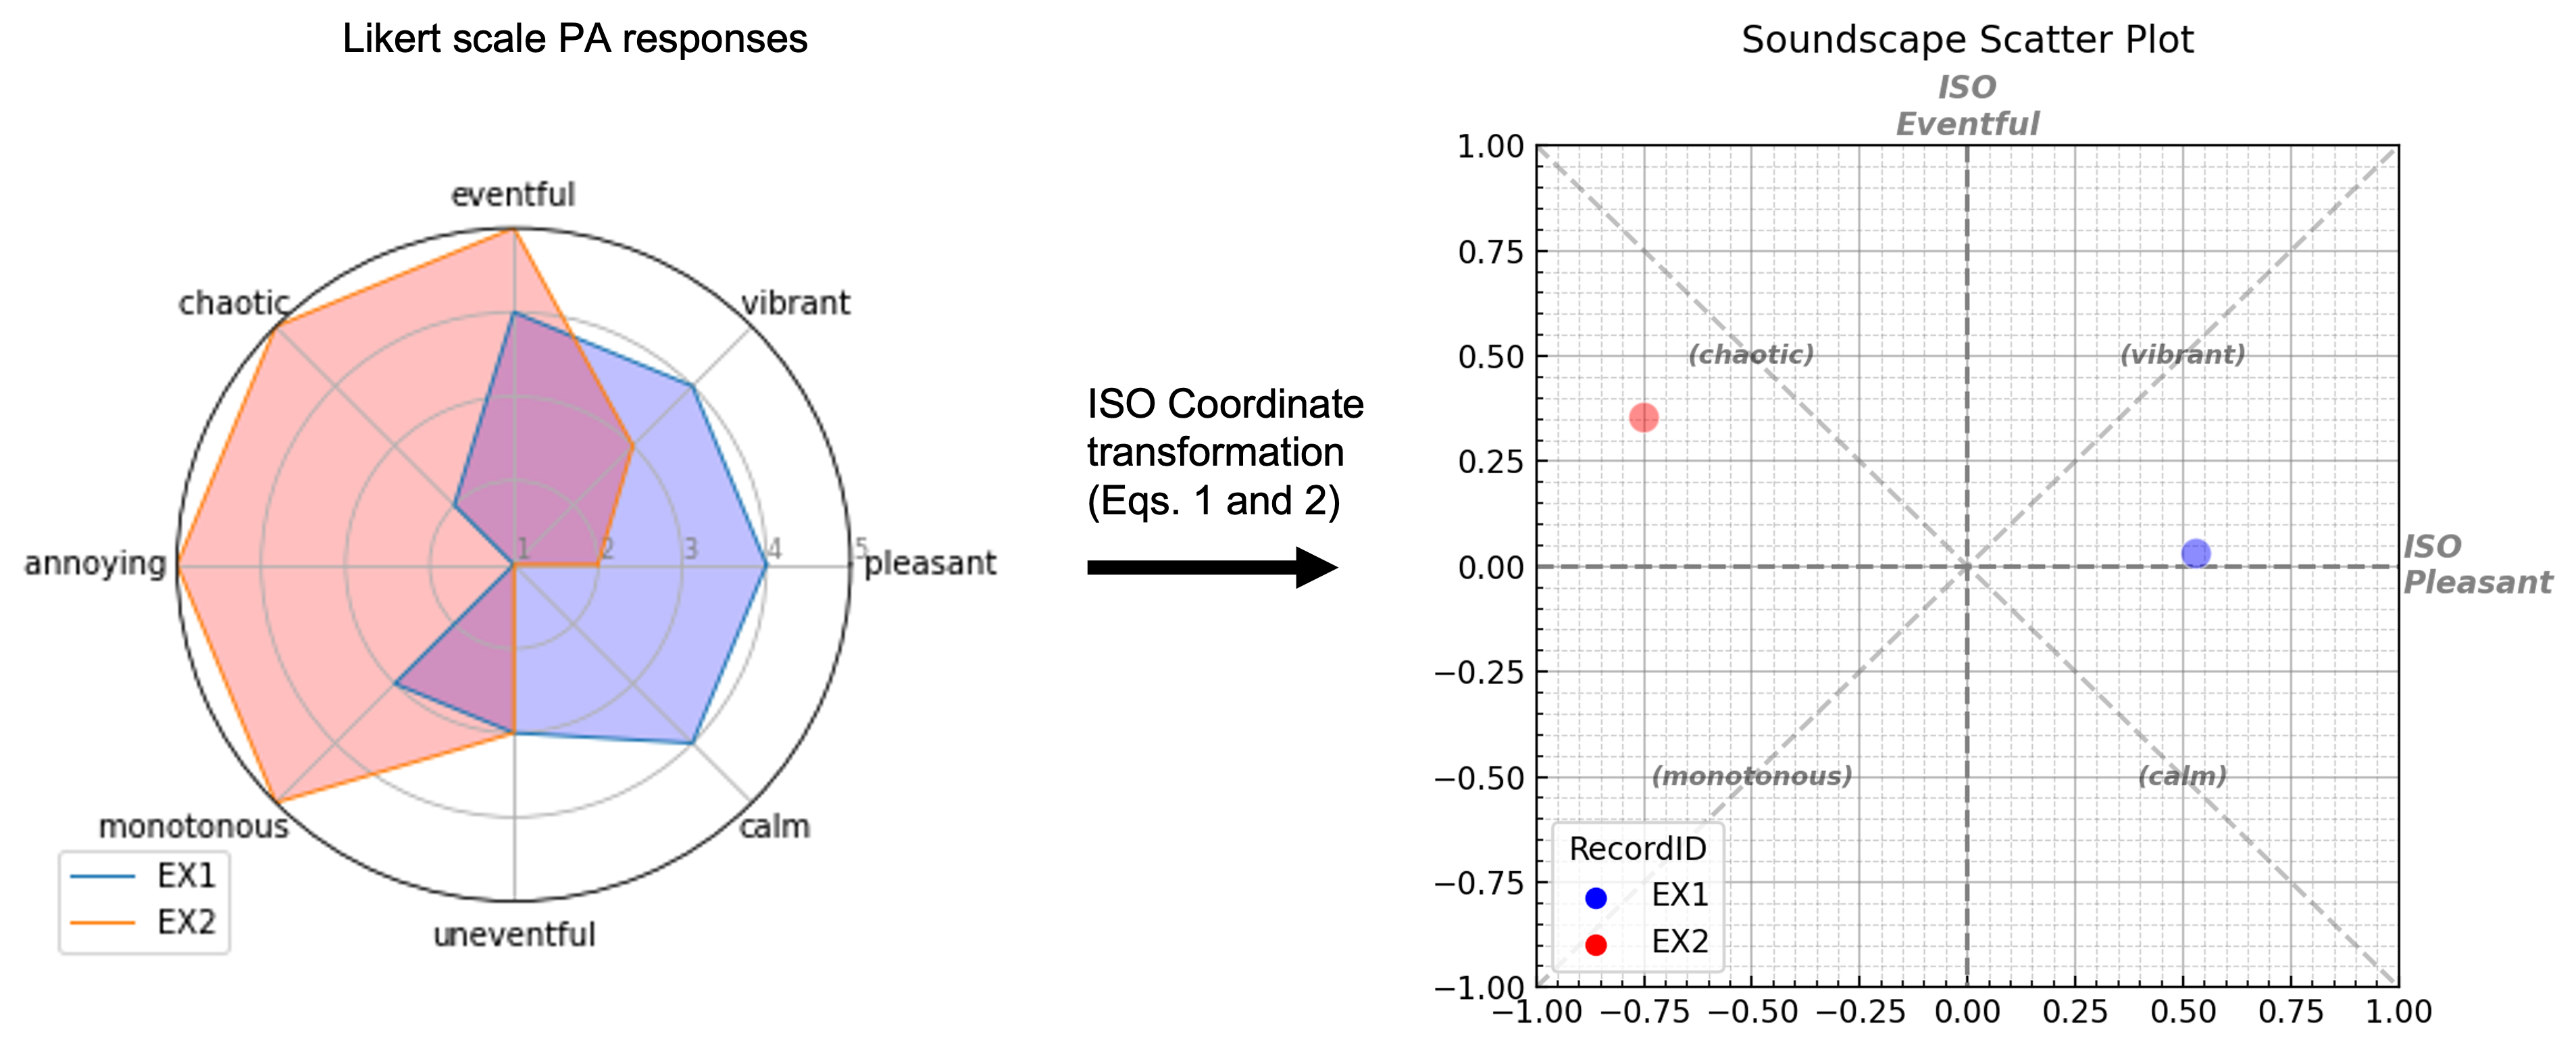
\includegraphics[width=\textwidth]{Figures/jasa-el_Figure1.png}
  \caption{Example of representations of two soundscape assessments. Left: Radar plot of two example perceptual attribute (PA) ratings on the Likert scales (1 to 5). Right: Scatter plot of the same assessments on the soundscape circumplex, transformed according to ISO 12913 Part 3.
    \label{fig:radar}
  }
\end{figure}

\subsection{Interpreting the Soundscape Circumplex}
%TODO:  \draft{Needs to be edited and connected to rest of chapter.}
%Move this paragraph to the interpretation of the circumplex section.
The circumplex model of soundscape, as originally defined by \citet{Axelsson2010principal}, is commonly understood to be a two-dimensional space (its main orthogonal components being annoying-pleasant and uneventful-eventful) where all regions of the space are equally likely to accommodate a given soundscape assessment \citep{Aletta2016Soundscape}. For instance, in theory, an extremely vibrant soundscape (e.g., with a score of 1) should be as likely to occur as an extremely annoying one, as well as one neutral on all dimensions (e.g., with a score of 0). However, a recent work by Lionello et al. \citep{Lionello2021Introducing} incidentally highlighted a possible issue with the process for representing soundscape assessments with the current ISO protocols. More specifically, when considering big numbers, soundscape assessments seem to have a bivariate normal distribution around the origin of the circumplex model. This would imply that not the whole space of the model is equally accessible to any given soundscape\footnote{\cref{app:CircCritique} offers a more in-depth critical critique and discussion of the specific consequences of this projection method in more detail than is appropriate to include here.}. Studies in the field show that data collection campaigns rarely return extreme values for soundscape dimensions \citep{Mancini2021Soundwalk} and so far the general interpretation has been that some soundscapes (e.g., extremely monotonous) may simply be difficult to find and detect with people in urban contexts \citep{Sun2019Classification}.

\subsection{Usefulness for predictive modelling}
This trigonometric projection method enables us to transform the 8 Likert scale PAQ values into a pair of coordinate values. This transformation has a few beneficial effects for applying standard modelling techniques to soundscape data. First, it simplifies and reduces the target problem; rather than needing to model eight separate responses, we are now focussed on only two. Second, it transforms the data from ordinal responses on a 1 to 5 scale into continuous values between -1 and +1. While it is clearly possible to model ordinal outputs through classification, the methods are often less familiar and more complicated than dealing with a more standard regression problem. For those outside of machine learning (i.e. designers, engineers, etc.) regression methods, especially linear regression, are already familiar and interpretable while methods of classification and ordinal modelling are typically less familiar. By applying the \gls{iso} projection to each individual's soundscape assessment, we generate a vector of output values which can be matched up to physical data measured for each individual. This creates the sort of input-output pair vector necessary for supervised regression learning.

\section{Machine Learning and Regression Techniques}
Machine learning approaches are typically divided into three broad categories: supervised, unsupervised, and reinforcement learning. In supervised learning, the training data consists of input-output pairs and learns a model which can map from the inputs to the outputs. In unsupervised learning, no corresponding output data is available to the training model, thus it learns patterns in the input without feedback. Reinforcement learning does not necessarily begin with training data, instead the learning agent is given a series of reinforcements in the form of rewards and punishments \citep{StuartRussell2021}. Reinforcement learning will not be used in this thesis. Unsupervised learning has been applied to a limited degree to the acoustic data collected in several sound environments which will be expanded upon in \cref{ch:lockdown}. 

The majority of this thesis is therefore focussed on creating a supervised learning model wherein the input data are the result of measurements and the output data are the perceptual assessments of the soundscapes. In the context of this thesis, there are two primary types of supervised machine learning models - regression and classification. Regression is applied when the output is a continuous number (e.g. temperature) whereas classification is used when the output is a discrete set of values. 



\subsection{Multi-level Linear Regression}

Multi-level regression modelling is a technique commonly used in fields such as psychology \citep{Quene2004multi,VolpertEsmond2021Using}, for applied prediction models \citep{Gelman2006Multilevel,Frees2006Multilevel}, and for a small number of previous soundscape studies \citep{Aumond2017Modeling}. \glspl{mlm} are particularly useful when data is organised at one or more levels or groups. As noted in \cref{tab:metadata}, the \gls{isd} forms a hierarchical structure with several groups nested within each other: Questionnaires within GroupIDs within SessionIDs within Locations, making a \gls{mlm} especially well-suited. The inherent grouped structure of the \gls{isd} necessitates a modelling and analysis approach which considers the differing relationships between the objective acoustic features and the soundscape's perceived affective quality ratings across the various locations and contexts. \glsplural{mlm} are also well-suited for engineering and design contexts as they are transparent, understandable, and conceptually familiar to most engineers. The concept behind \glspl{mlm} can be built up starting from simple linear regression, as given by:

\begin{equation}
  y_i = \alpha + \beta x_i + \epsilon
\end{equation}

For a classical multiple linear regression, we expand the $k$ coefficients out as so:

\begin{equation}
  \label{eqn:classicRegressModel}
  y_i = \alpha + \beta_1 x_{i1} + \ldots + \beta_k x_{ik} + \epsilon_i
\end{equation}

where:

\begin{itemize}
  \item \emph{i} indexes each unit, the smallest items of measurement. This is often a measurement per individual within a group or, in the \gls{isd} this can be for each recording.
  \item $y_i = (y_1, \ldots, y_n)$ the modelled outcome for each unit \emph{i};
  \item $k = 1, \dots, K$ denotes each of the multiple predictors;
  \item $\beta_k$ is the slope coefficient for the \emph{k\textsuperscript{th}} predictor;
\end{itemize}

Their primary feature of an \gls{mlm} is the ability to have coefficients and intercepts which are allowed to vary depending on the group \citep{DataAnalysisUsingGelman}. This can take three forms, which are illustrated in \cref{fig:GelmanMLM}:

\begin{enumerate}
  \item Varying intercepts
  \item Varying slopes
  \item Varying intercept and varying slopes
\end{enumerate}

\begin{figure}[h]
  \centering
  \begin{subfigure}[b]{.3\textwidth}
    \centering
    \caption{Varying intercepts}
    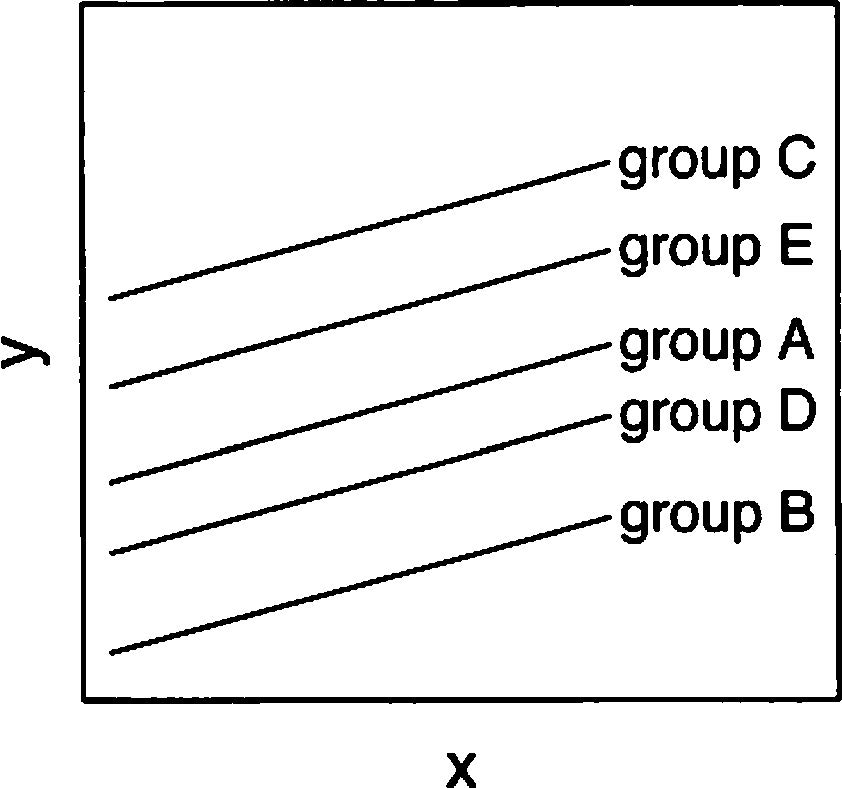
\includegraphics[width=\textwidth]{Figures/GelmanMLMa.jpg}    
  \end{subfigure}
\hfill
  \begin{subfigure}[b]{.3\textwidth}
    \centering
    \caption{Varying slopes}
    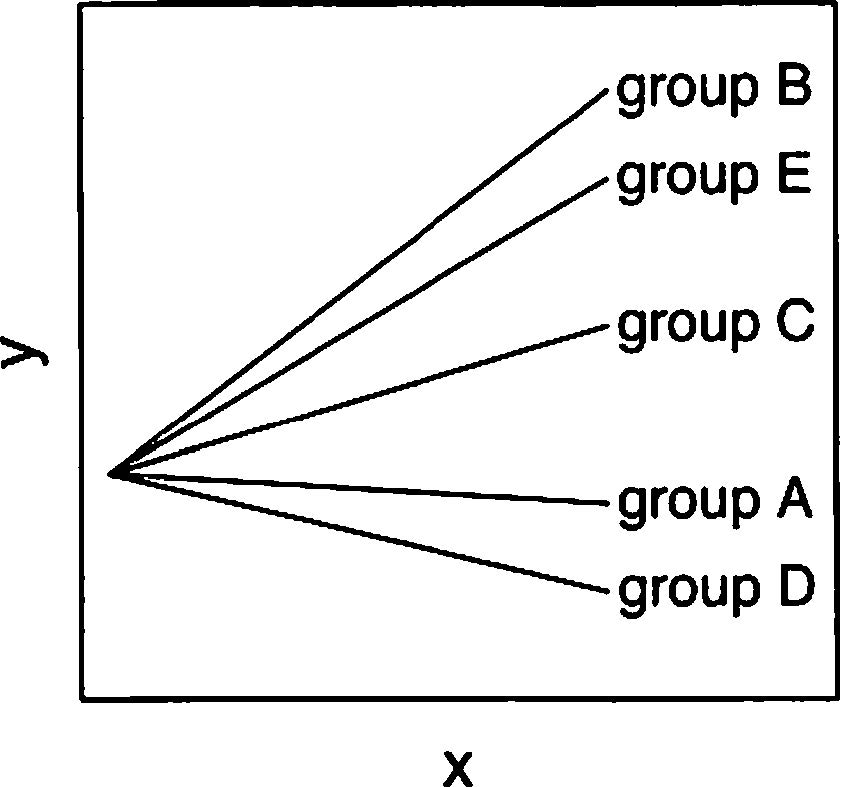
\includegraphics[width=\textwidth]{Figures/GelmanMLMb.jpg}    
  \end{subfigure}
\hfill
  \begin{subfigure}[b]{.3\textwidth}
    \centering
    \caption{Varying intercepts and slopes}
    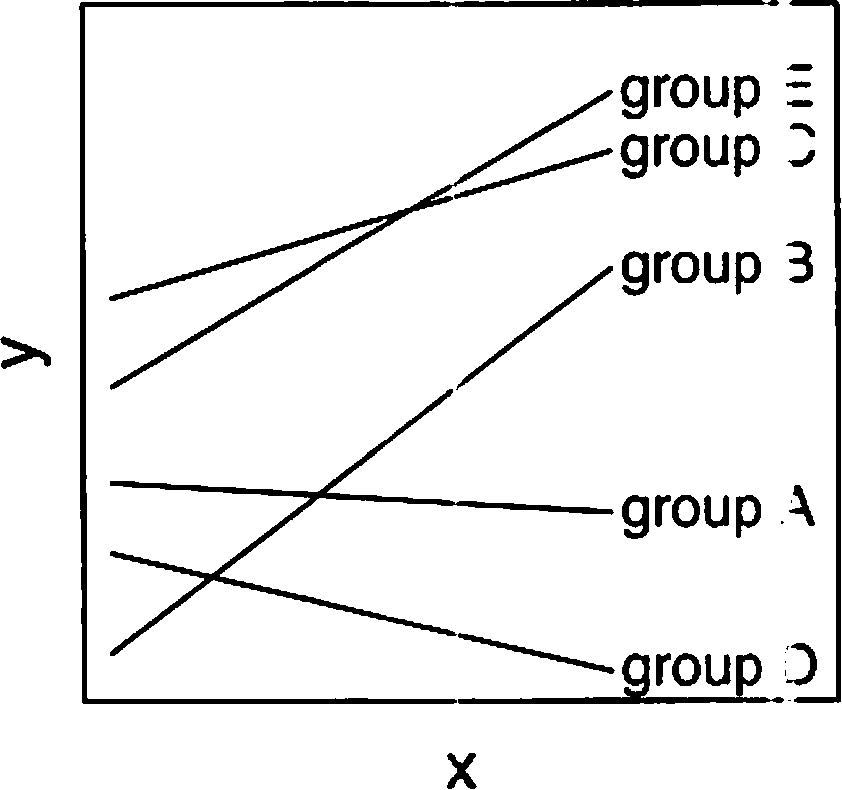
\includegraphics[width=\textwidth]{Figures/GelmanMLMc.jpg}    
  \end{subfigure}
  \hfill

  \caption{Linear regression model with with (a) varying intercepts ($y=\alpha_j + \beta x$), (b) varying slopes ($y=\alpha + \beta_j x$), (c) both ($y=\alpha_j + \beta_j x$). The varying intercepts correspond to group indicators as regression predictors, and the varying slopes represent interactions between \emph{x} and the group indicators. Reproduced with permission from \citet[Fig. 11.1]{DataAnalysisUsingGelman}. \label{fig:GelmanMLM}}
\end{figure}

In a varying intercept structure, the intercept for each input feature is allowed to vary according to the second level. This structure assumes that the linear relationship between each input feature and the output is consistent across the second level groups, but that the zero point (the intercept) is different. This is expressed mathematically \citep{DataAnalysisUsingGelman} as:

\begin{equation}
  %TODO: insert random intercept equation from Gelman 2006.
  y_i = \alpha_{j[i]} + \beta x + \epsilon{i}
\end{equation}

where groups are indexed by $j = , \ldots, J$, and \emph{j[i]} is the \emph{i\textsuperscript{th}} individual \emph{i} in group \emph{j}. This results in a vector of length \emph{J} containing one intercept result per group.

In the context of auditory perception studies, this is most appropriate for repeated measures experimental designs (as will be demonstrated in \cref{ch:mlmann}). A repeated measures study is one in which all participants experience all levels of the independent variables and provide some response in terms of the output variable. In other words, each participant constitutes a group in the model and they respond to all of the input variables \citep{Kristjansson2007Multilevel}. In this case, the \gls{mlm} framework is used to account for starting differences between respondents; populations are expected to demonstrate similar behaviours in response to a given stimulus, but may have differing initial starting points, i.e. different intercepts for each analysed feature. The \gls{mlm} framework using a varying intercept for each participant allows this initial difference among individuals to be accounted for while also highlighting the overall relationship between e.g. acoustic features and annoyance ratings for a given sound. 

Varying slope structures take the opposite assumption; each level shares the same intercept, while the coefficients for each feature are allowed to vary depending on the group. This assumes that different groups will have a different relationship between the input features and the output, but that these relationships may begin at a different threshold. This structure appears to be less commonly used than varying intercept models. This can be mathematically described as:

\begin{equation}
  %TODO: insert random slope equation from Gelman 2006
  y_i = \alpha + \beta_{j[i]}x_i + \epsilon_i
\end{equation}

where $\beta_{j[i]}$ is the slope coefficient for individual \emph{i} in group \emph{j}. 

With multiple predictors, we write:

\begin{equation}
  y_i = X_i B + \epsilon_i
\end{equation}

where B is a matrix of slope coefficients of size $J\times K$ with one coefficient for each predictor (\emph{k}) for each group (\emph{j}):

\[
  B_{J\times K} =
  \left[ {\begin{array}{cccc}
    \beta_{11} & \beta_{12} & \cdots & \beta_{1K}\\
    \beta_{21} & \beta_{22} & \cdots & \beta_{2K}\\
    \vdots & \vdots & \ddots & \vdots\\
    \beta_{J1} & \beta_{J2} & \cdots & \beta_{JK}\\
  \end{array} } \right]
\]

Finally, a varying-slope, varying-intercept model allows both the slope and intercept of the coefficients to vary for each group in the second level:

\begin{equation}
  y_i = \alpha_{j[i]} + \beta_{j[i]}x_i + \epsilon_i
\end{equation}

\paragraph*{Wilkinson-Rogers notation}
The analysis package used for constructing these models is \texttt{lme4} \citep{Bates2015Fitting} in the R statistical language \citep{RCT2018R}. This package makes use of a style of writing \glsplural{mlm} called Wilkinson-Rogers notation \citep{Wilkinson1973Symbolic}. Wilkinson-Rogers notation provides a way to specify \glsplural{mlm} without the need to specify coefficient values in a straightforward and easily readable way. For these models, the important operators to be familiar with are: $\sim$ indicates that a model regresses upon the dependent variable; $+$ sums the model terms;$\cdot$ indicates interaction terms; \texttt{(var|grp)} specifies a grouping variable or random effects term for an \gls{mlm}\footnote{It appears this notation was an extension of Wilkinson-Rogers introduced into the \texttt{nlme} R package by \citet{Pinheiro1997Graphical}.}. \cref{tab:wilkRog} shows some example models written in Wilkinson-Rogers notation:

\begin{table}[h]
\centering
\caption{Mathematical and Wilkinson-Rogers notation for several example models to demonstrate how to translate from one to the other. \texttt{var} is used to denote the independent variables to demonstrate that the variable name (e.g. \emph{loudness}) can be used directly in the notation. \label{tab:wilkRog}}
\resizebox{\linewidth}{!}{%
\begin{tabular}{lll} 
\toprule
\textbf{Description}                                                      & \textbf{Model}                                                                        & \textbf{Wilkinson-Rogers Notation}   \\
Two predictors                                                            & $y_i = \beta_0 + \beta_1 x_{i1} + \beta_2 x_{i2} + \epsilon_i$                        & \texttt{y $\sim$ var1 + var2}                 \\
\begin{tabular}[c]{@{}l@{}}Two predictors \\and no intercept\end{tabular} & $y_i = \beta_1 x_{i1} + \beta_2 x_{i2} + \epsilon_i$                                  & \texttt{y $\sim$ var1 + var2 - 1}             \\
\begin{tabular}[c]{@{}l@{}}Two predictors \\with interaction\end{tabular} & $y_i = \beta_0 + \beta_1 x_{i1} + \beta_2 x_{i2} + \beta_3 x_{i1}x_{i2} + \epsilon_i$ & \texttt{y $\sim$ var1 $\cdot$ var2}           \\
Varying intercept                                                          & $y_i = \alpha_{j[i]} + \beta_{x_i} + \epsilon_i$                                      & \texttt{y $\sim$ var1 + (1\textbar{}grp)}     \\
Varying slope                                                              & $y_i = \alpha + \beta_{j[i]x_i} + \epsilon_i$                                         & \texttt{y $\sim$ 1 + (var1\textbar{}grp)}     \\
\begin{tabular}[c]{@{}l@{}}Varying slope \\Varying intercept\end{tabular}   & $y_i = \alpha_{j[i]} + \beta_{j[i]x_i} + \epsilon_i$                                  & \texttt{y $\sim$ var1 + (var1\textbar{}grp)}  \\
\bottomrule
\end{tabular}
}
\end{table}

The structure inherent within the \gls{isd} means that this approach is particularly appropriate. In order to further demonstrate the structure and use of an \gls{mlm}, I'll further describe it in terms of the \gls{isd} data, where the most obvious second level for this \gls{mlm} is the location (a categorical variable defined by the LocationID). To demonstrate this, we'll specify a simple varying-intercept varying-slope \gls{mlm} which has the loudness (\gls{n5}) and sharpness (\gls{s}) as the two input variables, the recordings (taken per group in the \gls{isd} and indexed by the GroupID) make up the units at level 1, and the LocationID is level 2. 

\begin{equation}
  \label{eqn:basicISDMLM}
  \texttt{ISOpl $\sim$ loudness + sharpness + (loudness + sharpness | LocationID)}
\end{equation}

which would also be written as:

\begin{equation}
  ISOPl_i = \alpha_{j[i]} + \beta_{j[i]}N_{5_i} + \beta_{j[i]}S_i + \epsilon_i
\end{equation}

where $\alpha_{j[i]}$ is the mean \gls{isopl} score for LocationID \emph{j} where recording \emph{i} was taken and $\beta_{j[i]}N_5$ and $\beta_{j[i]}S$ are the loudness and sharpness slope coefficients for location \emph{j}. 

\paragraph*{Mixed effects: fixed and random effects} In some applications and fields, it is more common to refer to a \gls{mlm} as a \glsfirst{lmer}, however the two are simply different ways of speaking about the same mathematical concept \citep{Pinheiro2000Linear,DataAnalysisUsingGelman}. Although I typically refer to \glsplural{mlm}, I sometimes find it helpful to use the random-effects/fixed-effects terminology and \cref{ch:whostudy} primarily refers to the model as an \gls{lmer} since that work was targeted at a psychology audience, where mixed-effects is the more common term. In a varying-intercept varying-slope model, where certain features can be specified only at the unit level and others vary at the group level, the features at the unit level are considered \emph{fixed}: i.e. the relationship between independent and dependent variable remains fixed across all groups. In an \gls{lmer} the second level of effects are then termed the \emph{random effects}. This is useful -- particularly in a varying-intercept model -- where the effects in this second level are somewhat unexplainable. Consider a repeated measure study using a varying-intercept model: the grouping factor is the participant who has been exposed to multiple inputs. The second level operates to account for that participants consistent difference from the other participants, but that difference can be considered to be random for each participant, hence it is a \emph{random} effect when the goal is to elucidate the effects which are consistently seen across the sample. However, this use of the word random to refer to the second-level effects is not always useful, as highlighted by \citet[pg. 2]{DataAnalysisUsingGelman}. When we expect the grouping factor to have some explainable impact on the relationship between the independent and dependent variables (e.g. the context of the location has a complex, but non-random effect on the soundscape perception), then it is not appropriate to refer to it as `random'. 

In all, this concept helps to highlight the specific benefit of a \gls{mlm} approach. Conceptually, it would be possible to achieve a similar goal by treating the grouped data as `fully un-pooled' and to fit a separate linear regression model for each group. In the case of \cref{eqn:basicISDMLM}, we would treat the data from each location as a separate dataset and train a model on them each independently. This would reveal, within each location, the relationship between the loudness and sharpness of a sound and its perceived pleasantness. However, it would ignore the fact that there is a general, \emph{fixed}, relationship between loudness and pleasantness, regardless of the effects of the location.Alternatively, we could treat the data as `fully-pooled', creating a linear model with the form given in \cref{eqn:classicRegressModel} and only considers the fixed relationship across the entire dataset. A \gls{mlm}, which treats the data as `partially-pooled', and includes effects which are both fixed and can vary according to the location, enables us to investigate both the degree to which loudness generally impacts on pleasantness \emph{and} how this relationship changes according to the context of the location. 

\subsubsection{Structural Equation Models}

\gls{sem} is a statistical approach to testing hypotheses about relationships between variables and latent features which has been used by several studies in soundscape \citep{Tarlao2020Investigating,Hong2015Influence,Torresin2022Indoor}. \gls{sem} is a flexible approach in that it can include one or more independent or dependent variables and the variables can be continuous or discrete, factors or measured. As a collection of statistical methods, \gls{sem} is focussed on causal inference and is fundamentally built on a combination of path diagrams and regression modelling techniques \citep{Ullman2012Structural}. Most frequently in an \gls{sem}, the researcher constructs a path diagram (often called \glsplural{dag}) which expresses the hypothesised relationships between the variables of interest. These path diagrams can be quite complex, including covariance relationships, latent variables, residuals, and distinctions between factors and measured variables. The model is then fit to the data through a selected estimation method (most typically Maximum likelihood (ML) as in regression modelling) and evaluated. The model may then be further reduced or modified if necessary. \gls{sem} also allows for multilevel modelling where separate models are developed for different levels of a nested hierarchy. This is conceptually equivalent to the \gls{mlm} or \gls{lmer} discussed throughout this thesis. Several studies in the soundscape literature have made use of \gls{sem}. 


 \subsection{Feature Selection}
 \label{sec:featureSelection}
In general, throughout this thesis, two models are built separately: one for predicting \gls{isopl} and one for predicting \gls{isoev}. A separate backwards-step feature selection was performed for each of the outcome models in order to identify the minimal feature set to be used for predicting each outcome. In this feature selection process, an initial model containing all of the candidate features was fit. Each feature was then removed from the model one at a time, then the best-performing model is selected and the procedure continues step-wise until no improvement is seen by removing more features. This process is carried out first on the location-level features (including the potential to remove all features including LocationID, resulting in a `flat' or standard multivariate linear regression model), then on the individual-level features.  To check for multicollinearity among the selected features, the \gls{vif} was calculated and a threshold of $\gls{vif} < 5$ was set. Any features which remained after the backwards step-wise selection and which exceeded this threshold were investigated and removed if they were highly collinear with the other features.

   The model fitting and feature selection was performed using the \texttt{step} function from \texttt{lmerTest} (v3.1.3) \citep{Kuznetsova2017lmerTest} in R statistical software (v.4.0.3) \citep{RCT2018R}. The summaries and plots were created using the \texttt{sjPlot} package (v.2.8.6) \citep{Luedecke2021sjPlot} and \texttt{seaborn} (v.0.11.1) \citep{Waskom2021seaborn}.

  %  \subsubsection{Mutual Information}
  %  \draft{It appears that mutual information is related to the Bayes formula. I still need to read more into this, but it appears based on relative and overlapping probability distributions between the variables in question.}
  %  \paragraph*{From scholarpedia:}
  %  % http://www.scholarpedia.org/article/Mutual_information
  %  \draft{Based on entropy, where the uncertainty about a variable can be expressed as "the number of yes/no questions it takes to guess a random variable, given knowledge of the underlying distribution and taking the optimal question-asking strategy". "The mutual information is therefore the \emph{reduction} in uncertainty about variable $X$, or the expected reduction in the number of yes/no questions needed to guess $X$ after observing $Y$.". }

  %  \draft{"Mutual Information is just one way among many of measuring how related two variables are. However, it is a measure ideally suited for analyzing communication channels. Abstractly, a communication channel can be visualized as a transmission medium which receives an input $x$ and produces an output $y$. If the channel is \emph{noiseless}, the output will be equal to the input. However, in general, the transmission medium is noisy and an input $x$ is converted to an output $y$ with probability $P_{Y|X}(y|x)$. }
  %  \misc{This seems very useful for my conception of sound perception / auditory processing, where the perception system is a noisy communication channel.}

  %  \subsubsection{Conditional Mutual Information}
  %  The Mutual Information between two variables, given another variable as a control.

%  \subsection{Clustering Analysis}
%    \paragraph{K-means}
%    \paragraph{nbclust}
